%%%%%%%%%%%%%%%%%%%%%%%%%%%%%%%%%%%%%%%%%%%%%%%%%%%%%%%%%%%%%%%%%%%%%%%%%%%
%% This file is part of the book
%%
%% Sage for High School
%% http://code.google.com/p/high-school-sage/
%%
%% Copyright (C) 2010 Minh Van Nguyen <nguyenminh2@gmail.com>
%%
%% See the file COPYING for copying conditions. See the file LICENSE
%% for the terms under which the whole book is licensed.
%%%%%%%%%%%%%%%%%%%%%%%%%%%%%%%%%%%%%%%%%%%%%%%%%%%%%%%%%%%%%%%%%%%%%%%%%%%

\documentclass[a4paper,twoside,12pt]{book}

\usepackage{mystyle}

\begin{document}

\pagenumbering{alph}

\title{\Huge\bf Sage for High School}
\author{\Large Minh Van Nguyen}
\date{%
  Version~\documentEdition \\
  \today
}
\maketitle

%% Copyright page
{\thispagestyle{empty}
  \noindent Copyright \copyright\ 2010 \\
Minh Van Nguyen \url{<nguyenminh2@gmail.com>} \\\\
Permission is granted to copy, distribute and/or modify this document
under the terms of the GNU Free Documentation License, Version 1.3
or any later version published by the Free Software Foundation;
with no Invariant Sections, no Front-Cover Texts, and no
Back-Cover Texts. A copy of the license is included in the section
entitled ``GNU Free Documentation License''. \\

\noindent
The latest version of the book is available from its website at \\

\url{http://code.google.com/p/high-school-sage/}
 \\\\
  \textbf{Edition} \\
  Version~\documentEdition \\
  \today
}

%% front matter
\frontmatter
%% Setting the TOC depth: only list chapters and sections
\setcounter{tocdepth}{1}
\tableofcontents
\let\cleardoublepage\clearpage
\listoffigures
\addcontentsline{toc}{chapter}{List of Figures}
\let\cleardoublepage\clearpage

%% main document body
\mainmatter
%%%%%%%%%%%%%%%%%%%%%%%%%%%%%%%%%%%%%%%%%%%%%%%%%%%%%%%%%%%%%%%%%%%%%%%%%%%

\chapter{Algebraic Simplification}

\begin{enumerate}
\item Simplifying algebraic expressions using the distributive laws:
  \begin{enumerate}
  \item binomial expansion: $(a + b)(c + d) = ac + ad + bc + bd$

  \item difference of two squares: $(a + b)(a - b) = a^2 - b^2$

  \item perfect squares: $(a + b)^2 = a^2 + 2ab + b^2$ and
    $(a - b)^2 = a^2 - 2ab + b^2$

  \item perfect cubes

  \item sum and difference of two cubes
  \end{enumerate}

\item Simplifying rational expressions:
  \begin{enumerate}
  \item addition of rational expressions

  \item subtraction of rational expressions

  \item multiplication of rational expressions

  \item division of rational expressions
  \end{enumerate}
\end{enumerate}


%%%%%%%%%%%%%%%%%%%%%%%%%%%%%%%%%%%%%%%%%%%%%%%%%%%%%%%%%%%%%%%%%%%%%%%%%%%

\section{Collect like terms}
\index{like terms}

In simplifying an algebraic expression, a basic technique is
identifying like terms\index{like terms}, simplify them and in the
process we also simplify the whole expression. Two like terms can be
simplified to one term because only like terms can be added or
subtracted. The expression
%
\begin{equation}
\label{eq:algebraic_simplify:has_like_terms}
5x + 12x + 17y
\end{equation}
%
can be simplified because $5x$ and $12x$ are like
terms. Contrast~(\ref{eq:algebraic_simplify:has_like_terms}) with
\[
3x + 7y
\]
which has no like terms and cannot be simplified any further.

\begin{lstlisting}
sage: x, y = var("x, y")
sage: 5*x + 12*x + 17*y
17*x + 17*y
sage: simplify(5*x + 12*x + 17*y)
17*x + 17*y
sage: 3*x + 7*y
3*x + 7*y
sage: simplify(3*x + 7*y)
3*x + 7*y
sage: a, b, m, n = var("a, b, m, n")
sage: a + b^2 - 4*a*b + 3*a - b^2 - 2*a*b
-6*a*b + 4*a
sage: 3*(x^2)*(y^3) + 4*x*(y^2) - 9*(y^3)*(x^2) - 7*(y^2)*x
-6*x^2*y^3 - 3*x*y^2
\end{lstlisting}

%%%%%%%%%%%%%%%%%%%%%%%%%%%%%%%%%%%%%%%%%%%%%%%%%%%%%%%%%%%%%%%%%%%%%%%%%%%
%% This file is part of the book
%%
%% Sage for High School
%% http://code.google.com/p/high-school-sage/
%%
%% Copyright (C) 2010 Minh Van Nguyen <nguyenminh2@gmail.com>
%%
%% See the file COPYING for copying conditions. See the file LICENSE
%% for the terms under which the whole book is licensed.
%%%%%%%%%%%%%%%%%%%%%%%%%%%%%%%%%%%%%%%%%%%%%%%%%%%%%%%%%%%%%%%%%%%%%%%%%%%

\chapter{Surds, Powers, and Logarithms}

\begin{enumerate}
\item Simplifying expressions involving surds:
  \begin{enumerate}
  \item addition of surds

  \item subtraction of surds

  \item multiplication of surds

  \item division of surds

  \item rationalizing the denominator
  \end{enumerate}

\item Powers
  \begin{enumerate}
  \item addition of powers

  \item subtraction of powers

  \item multiplication of powers

  \item negative powers

  \item fractional powers
  \end{enumerate}

\item Logarithms: expressing huge numbers in scientific notation
\end{enumerate}

%%%%%%%%%%%%%%%%%%%%%%%%%%%%%%%%%%%%%%%%%%%%%%%%%%%%%%%%%%%%%%%%%%%%%%%%%%%
%% This file is part of the book
%%
%% Sage for High School
%% http://code.google.com/p/high-school-sage/
%%
%% Copyright (C) 2010 Minh Van Nguyen <nguyenminh2@gmail.com>
%%
%% See the file COPYING for copying conditions. See the file LICENSE
%% for the terms under which the whole book is licensed.
%%%%%%%%%%%%%%%%%%%%%%%%%%%%%%%%%%%%%%%%%%%%%%%%%%%%%%%%%%%%%%%%%%%%%%%%%%%

\chapter{Number Theory}


%%%%%%%%%%%%%%%%%%%%%%%%%%%%%%%%%%%%%%%%%%%%%%%%%%%%%%%%%%%%%%%%%%%%%%%%%%%

\section{Integers}
\index{integer}

An \emph{integer}\index{integer} is a whole number. It can be
positive, negative, or zero. Examples of integers include $-13$, $-1$,
$0$, and $42$. When we talk about all the whole numbers, we can use
the name \emph{integer}\index{integer} to refer to them, or we can
list all the whole numbers like so:
\[
\dots, -4, -3, -2, -1, 0, 1, 2, 3, 4, \dots
\]
But for convenience, we usually write $\ZZ$\index{$\ZZ$} to denote the
set of all integers:
\[
\ZZ
=
\{\dots, -3, -2, -1, 0, 1, 2, 3, \dots\}.
\]
In Sage, the set of all integers is represented as \verb!ZZ! and a
single integer is represented using \verb!Integer!:
%
\begin{lstlisting}
sage: ZZ
Integer Ring
sage: type(ZZ)
<type 'sage.rings.integer_ring.IntegerRing_class'>
sage: 1 in ZZ
True
sage: -1 in ZZ
True
sage: 3.1415 in ZZ
False
sage: type(3)
<type 'sage.rings.integer.Integer'>
sage: Integer
<type 'sage.rings.integer.Integer'>
\end{lstlisting}
%
Notice that in the above code listing, we used \verb!in! to test
whether or not a number is an integer. The command
%
\begin{lstlisting}
sage: 1 in ZZ
True
\end{lstlisting}
%
gives the result \verb!True! because $1$ is an integer. On the other
hand, the command
%
\begin{lstlisting}
sage: 3.1415 in ZZ
False
\end{lstlisting}
%
gives \verb!False! because $3.1415$ is not an integer.


%%%%%%%%%%%%%%%%%%%%%%%%%%%%%%%%%%%%%%%%%%%%%%%%%%%%%%%%%%%%%%%%%%%%%%%%%%%

\section{Prime numbers}
\index{prime}

A positive integer $n > 1$ is a \emph{prime}\index{prime} number if
its factors are exclusively $1$ and itself. The integer $2$ is prime
because its only factors are $1$ and $2$. As a matter of fact, $2$ is
the smallest prime integer. The next prime after $2$ is $3$. However,
the next integer $4$ is not prime because $2$ is a factor of $4$. In
Sage, the command \verb!is_prime! tests whether or not an integer is
prime. We can obtain the first $15$ prime numbers using the command
\verb!primes_first_n!.

\begin{lstlisting}
sage: is_prime(1)
False
sage: is_prime(2)
True
sage: is_prime(3)
True
sage: is_prime(4)
False
sage: primes_first_n(15)
[2, 3, 5, 7, 11, 13, 17, 19, 23, 29, 31, 37, 41, 43, 47]
\end{lstlisting}

If $n$ is an integer, the command \verb!next_prime! can be used to
compute the next prime integer starting from $n$. Likewise, the command
\verb!previous_prime! computes the previous prime integer starting
from $n$.
%
\begin{lstlisting}
sage: next_prime(-25)
2
sage: next_prime(1)
2
sage: next_prime(50)
53
sage: previous_prime(50)
47
sage: previous_prime(3)
2
sage: previous_prime(2)
Traceback (most recent call last):
...
ValueError: no previous prime
\end{lstlisting}
%
The command
%
\begin{lstlisting}
sage: next_prime(-25)
2
\end{lstlisting}
%
results in \verb!2! because $2$ is the smallest prime. In other words,
there are no primes smaller than $2$, which explains the result of the
following command:
%
\begin{lstlisting}
sage: previous_prime(2)
Traceback (most recent call last):
...
ValueError: no previous prime
\end{lstlisting}

There are various questions we can ask about prime\index{prime}
numbers. For example, how many prime integers are there? Over two
thousand years ago, the Greek mathematician Euclid\index{Euclid}
proved that there are infinitely many primes. No matter how high up we
count, there is still a prime number to be found.

Here's another question: If $n$ is a positive integer greater than
$1$, how many primes are there between $1$ and $n$? In the case of
$n = 50$, we could use the command \verb!primes_first_n! to list the
first 20 primes, then count how many of those primes are less than or
equal to $50$.
%
\begin{lstlisting}
sage: primes_first_n(20)
[2, 3, 5, 7, 11, 13, 17, 19, 23, 29, 31, 37, 41, 43, 47, 53, 59, 61, 67, 71]
sage: P = [2, 3, 5, 7, 11, 13, 17, 19, 23, 29, 31, 37, 41, 43, 47]; P
[2, 3, 5, 7, 11, 13, 17, 19, 23, 29, 31, 37, 41, 43, 47]
sage: len(P)
15
\end{lstlisting}
%
In the above code listing, we put all the primes less than or equal to
$50$ into the list \verb!P!. We then used the command \verb!len! to
obtain the length of that list. From the above output, there are $15$
primes less than or equal to $n = 50$.

Alternatively, we can let the command \verb!prime_pi!\index{$\pi(x)$}
do all the hard work for us. Given an integer $n$---either positive,
negative, or zero---the command \verb!prime_pi(n)! counts how many
primes are less than or equal to $n$.
%
\begin{lstlisting}
sage: prime_pi(50)
15
sage: prime_pi(100)
25
sage: prime_pi(1000)
168
sage: prime_pi(10000)
1229
sage: prime_pi(0)
0
sage: prime_pi(-10)
0
\end{lstlisting}
%
To study the output of \verb!prime_pi(n)!\index{$\pi(x)$} as the
integer \verb!n! increases, we could substitute $n = 1, 2, 3, \dots$
into the command. Or we could use \verb!plot! together with
\verb!prime_pi! to visualize how the output of \verb!prime_pi! changes
as $n$ increases in
value. Figure~\ref{fig:number_theory:prime_pi_for_n_leq_100}
illustrates the change in the values of \verb!prime_pi! as $n$ takes
on all integer values from $0$ up to and including $100$. Notice that
when $n = 50$, the output of \verb!prime_pi! is $15$, which confirms
our computation above. The horizontal axis shows integer values of $n$
from $0$ to $100$, inclusive, while the vertical axis shows the output
of the command \verb!prime_pi(n)!. The figure was produced using the
following code listing:
%
\begin{lstlisting}
sage: P = plot(prime_pi, 0, 100)
sage: V = line([(50,0), (50,25)], color="red")     # vertical line
sage: H = plot(15, xmin=0, xmax=100, color="red")  # horizontal line
sage: P + H + V
\end{lstlisting}
%
\begin{figure}[!htbp]
\centering
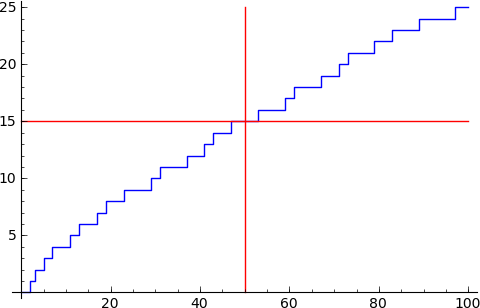
\includegraphics[scale=0.8]{images/prime-pi-100}
\caption{Values of \texttt{prime\_pi(n)} for $n = 0, 1, 2, \dots, 100$.}
\label{fig:number_theory:prime_pi_for_n_leq_100}
\end{figure}
%
And Figure~\ref{fig:number_theory:prime_pi_for_n_leq_1000} shows the
behavior of \verb!prime_pi! as $n$ increases from $0$ to $1000$. The
figure was produced using the command:
%
\begin{lstlisting}
sage: plot(prime_pi, 0, 1000)
\end{lstlisting}
%
\begin{figure}[!htbp]
\centering
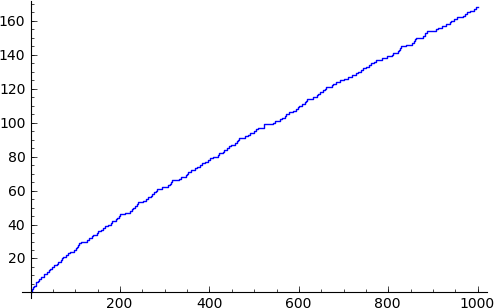
\includegraphics[scale=0.8]{images/prime-pi-1000}
\caption{Values of \texttt{prime\_pi(n)} for $n = 0, 1, 2, \dots, 1000$.}
\label{fig:number_theory:prime_pi_for_n_leq_1000}
\end{figure}


%%%%%%%%%%%%%%%%%%%%%%%%%%%%%%%%%%%%%%%%%%%%%%%%%%%%%%%%%%%%%%%%%%%%%%%%%%%

\section{Divisibility}
\index{divisibility}

For any two integers $a$ and $n$, we say that $a$
\emph{divides}\index{divides} $n$ if $a$ is a factor of $n$. That is,
if we can find an integer $b$ such that $n = ab$, then $a$ is a
factor\index{factor} of $n$. In that case, $b$ is also a factor of
$n$. The integer $2$ divides, or is a factor of, $4$ because
$4 = 2 \times 2$. Similarly, both $2$ and $3$ are factors of, or both
divide, $6$ because $6 = 2 \times 3$.

Does every positive integer have a factor\index{factor}? Yes. In fact,
if $n > 1$ is an integer, then $n$ has a factor that is greater than
$1$. We can make a stronger claim: Every integer $n > 1$ has a prime
factor. A factorization, or prime factorization, of $n$ is product
containing all the primes that divide $n$. Examples of prime
factorizations include $4 = 2 \times 2$ and $6 = 2 \times 3$. However,
$8 = 2 \times 4$ is not a prime factorization of $8$ because the
product $2 \times 4$ has $4$, which is not prime.

To find all the positive divisors\index{divisor} of an integer, use
the command \verb!divisors!.
%
\begin{lstlisting}
sage: divisors(4)
[1, 2, 4]
sage: divisors(6)
[1, 2, 3, 6]
sage: divisors(8)
[1, 2, 4, 8]
\end{lstlisting}
%
To write $n$ as a product of primes, use \verb!factor!.

\begin{lstlisting}
sage: factor(4)
2^2
sage: factor(6)
2 * 3
sage: factor(8)
2^3
\end{lstlisting}


%%%%%%%%%%%%%%%%%%%%%%%%%%%%%%%%%%%%%%%%%%%%%%%%%%%%%%%%%%%%%%%%%%%%%%%%%%%

\section{Greatest common divisors}
\index{greatest common divisor}

Let $a$ and $b$ be integers, not both zero. The
\emph{greatest common divisor}\index{greatest common divisor}
(GCD)\index{GCD} of $a$ and $b$ is the largest positive integer which
is a factor of both $a$ and $b$. We use $\gcd(a,b)$ to denote this
largest positive factor. If $n$ is any positive integer, then
$\gcd(n, 0) = n = \gcd(0, n)$. If $a$ and $b$ are both zero, then we
define their GCD to be $\gcd(0,0) = 0$. The GCD\index{GCD} of any two
distinct primes is $1$, and the GCD of $18$ and $27$ is $9$.
%
\begin{lstlisting}
sage: gcd(0, 0)
0
sage: gcd(12, 0)
12
sage: gcd(13, 0)
13
sage: N = [1..20]; N
[1, 2, 3, 4, 5, 6, 7, 8, 9, 10, 11, 12, 13, 14, 15, 16, 17, 18, 19, 20]
sage: G = []
sage: for i in N:
...       G.append(gcd(i, 0))
sage: N
[1, 2, 3, 4, 5, 6, 7, 8, 9, 10, 11, 12, 13, 14, 15, 16, 17, 18, 19, 20]
sage: G
[1, 2, 3, 4, 5, 6, 7, 8, 9, 10, 11, 12, 13, 14, 15, 16, 17, 18, 19, 20]
\end{lstlisting}
%
In the above code listing, we used the command \verb![1..20]! to
obtain a list of all integers from $1$ to $20$, inclusive.

To find the GCD of $18$ and $27$, we could first use \verb!divisors!
to find the set of all positive divisors of each integer. We then
compare the set of divisors for $18$ with that for $27$, picking out
any integers that are common to both sets. From among all the divisors
that are common to both $18$ and $27$, we choose the largest such
divisor. The result is the GCD of $18$ and $27$.
%
\begin{lstlisting}
sage: D18 = Set(divisors(18)); D18
{1, 2, 3, 6, 9, 18}
sage: D27 = Set(divisors(27)); D27
{3, 1, 27, 9}
sage: D = D18.intersection(D27); D
{1, 3, 9}
sage: max(D)
9
\end{lstlisting}
%
The output of \verb!divisors! is a list. We used the command
\verb!Set!\index{set} to convert the result of \verb!divisors! into a
set. We then used \verb!intersection!\index{intersection} to produce
the intersection of the two sets \verb!D18! and \verb!D27!; this
intersection is the set \verb!D!. Finally, we used \verb!max! to
compute the maximum element in the set \verb!D!, i.e. $9$, the GCD we
require.

Sage uses \verb!gcd(a, b)! to denote the GCD of $a$ and $b$. The GCD
of any two integers can be computed as follows:
%
\begin{lstlisting}
sage: gcd(3, 59)
1
sage: gcd(18, 27)
9
\end{lstlisting}

What about the case where any of $a$ and $b$ is negative? For example,
how do we compute the GCD of $-18$ and $27$, or $\gcd(-18, -27)$? If
$a$ is negative, for example, then we compute its
\emph{absolute value}\index{absolute value} and use that value to find
the GCD of $a$ and $b$. The absolute value of a number $x$ is written
as $|x|$ and is defined as
\[
|x|
=
\begin{cases}
x, & \text{if $x \geq 0$}, \\
-1 \times x, & \text{if $x < 0$}.
\end{cases}
\]
For example, the absolute value of $27$ is $|27| = 27$ because
$27 \geq 0$; the absolute value of $-18$ is
$|-18| = -1 \times (-18) = 18$ because $-18$ is negative. Then the GCD
of $-18$ and $27$ is
%
\begin{align*}
\gcd(-18, 27)
&=
\gcd(|-18|, 27) \\
&=
\gcd(18, 27) \\
&=
9.
\end{align*}

\begin{lstlisting}
sage: gcd(18, 27)
9
sage: gcd(-18, 27)
9
sage: gcd(-18, -27)
9
sage: # positive values of a, with b = 27
sage: N = [1..10]; N
[1, 2, 3, 4, 5, 6, 7, 8, 9, 10]
sage: G = []
sage: for i in N:
...       G.append(gcd(i, 27))
sage: G
[1, 1, 3, 1, 1, 3, 1, 1, 9, 1]
sage: # negative values of a, with b = 27
sage: N = [-1..-10, step=-1]; N
[-1, -2, -3, -4, -5, -6, -7, -8, -9, -10]
sage: G = []
sage: for i in N:
...       G.append(gcd(i, 27))
sage: G
[1, 1, 3, 1, 1, 3, 1, 1, 9, 1]
\end{lstlisting}

Figure~\ref{fig:number_theory:gcd_n_27} plots $\gcd(n, 27)$ for
integer values of $n$ from $1$ to $100$, inclusive. The horizontal
axis shows the values of $n$, while the vertical axis shows the values
of $\gcd(n, 27)$.

\begin{figure}[!htbp]
\centering
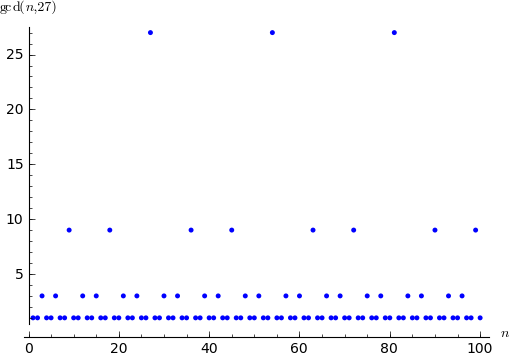
\includegraphics[scale=1.0]{images/gcd-100}
\caption{The GCD of $n$ and $27$ for $n = 1, 2, \dots, 100$.}
\label{fig:number_theory:gcd_n_27}
\end{figure}


%%%%%%%%%%%%%%%%%%%%%%%%%%%%%%%%%%%%%%%%%%%%%%%%%%%%%%%%%%%%%%%%%%%%%%%%%%%

\subsection{Relatively prime integers}
\index{relatively prime}
\index{coprime}

If $\gcd(a,b) = 1$, we say that $a$ is
\emph{coprime}\index{coprime}~(or relatively
prime\index{relatively prime}) to $b$.  In particular,
$\gcd(3, 59) = 1$ so $3$ is coprime to $59$ and vice versa.

Consider all the integers from $1$ to $20$, inclusive.  List all those
integers that are coprime to $20$.  In other words, find those
integers $n$, where $1 \leq n \leq 20$, such that
$\gcd(n,20) = 1$. The latter task can be easily accomplished with a
little bit of Sage programming:

\begin{lstlisting}
sage: for n in range(1, 21):
...       if gcd(n, 20) == 1:
...           print(n),
1 3 7 9 11 13 17 19
\end{lstlisting}

The above commands can be placed inside a function called
\verb!my_phi20! to save the hassle of retyping them every time we want
to use those exact commands.\index{Euler phi function}

\begin{lstlisting}
sage: def my_phi20():
...       for n in range(1, 21):
...           if gcd(n, 20) == 1:
...               print(n),
sage: my_phi20()
1 3 7 9 11 13 17 19
\end{lstlisting}
%
From the output of \verb!my_phi20!, note that there are $8$ integers
between $1$ and $20$, inclusive, that are coprime to $20$. Without
explicitly generating the list
%
\begin{equation}
\label{eq:integers_coprime_to_20}
1 \quad 3 \quad 7 \quad 9 \quad 11 \quad 13 \quad 17 \quad 19
\end{equation}
%
how can we compute the number of integers between $1$ and $20$,
inclusive, that are coprime to $20$? We could modify our function
\verb!my_phi20! so that it finds the number of positive integers that
are coprime to a given integer $n$.

\begin{lstlisting}
sage: def my_phi(n):
...       coprime = []
...       for i in range(1, n+1):
...           if gcd(i, n) == 1:
...               coprime.append(i)
...       return len(coprime)
sage: my_phi(20)
8
sage: my_phi(50)
20
sage: my_phi(100)
40
\end{lstlisting}

Alternatively, we could use the
\emph{Euler phi function}\index{Euler phi function}
$\varphi(n)$\index{$\varphi(n)$}, whose corresponding Sage built-in
function is \verb!euler_phi!.

\begin{lstlisting}
sage: euler_phi(20)
8
sage: euler_phi(50)
20
sage: euler_phi(100)
40
\end{lstlisting}


%%%%%%%%%%%%%%%%%%%%%%%%%%%%%%%%%%%%%%%%%%%%%%%%%%%%%%%%%%%%%%%%%%%%%%%%%%%

\section{Least common multiples}
\index{least common multiple}
\index{LCM}

Let $a$ and $b$ be integers, both of which are not zero. The
\emph{least common multiple}\index{least common multiple}
(LCM\index{LCM}) of $a$ and $b$ is the smallest positive integer which
is a multiple of both $a$ and $b$. We write the least common multiple
of $a$ and $b$ as $\lcm(a, b)$. If $n$ is any integer, then $\lcm(n,
0) = 0$ and $\lcm(0, n) = 0$. Where $a$ and $b$ are both zero, then
$\lcm(0,0) = 0$.

\begin{lstlisting}
sage: lcm(0, 0)
0
sage: lcm(13, 0)
0
sage: lcm(42, 0)
0
sage: N = [1..20]; N
[1, 2, 3, 4, 5, 6, 7, 8, 9, 10, 11, 12, 13, 14, 15, 16, 17, 18, 19, 20]
sage: L = []
sage: for i in N:
...       L.append(lcm(i, 0))
sage: N
[1, 2, 3, 4, 5, 6, 7, 8, 9, 10, 11, 12, 13, 14, 15, 16, 17, 18, 19, 20]
sage: L
[0, 0, 0, 0, 0, 0, 0, 0, 0, 0, 0, 0, 0, 0, 0, 0, 0, 0, 0, 0]
\end{lstlisting}

To compute the LCM of two integers $a$ and $b$, both of which are not
zero, first compute the GCD of $a$ and $b$. Finally, divide $ab$ by
$\gcd(a,b)$. This procedure is summarized in the following formula:
%
\begin{equation}
\label{eq:number_theory:formula_for_LCM}
\lcm(a, b)
=
\frac{ab}{\gcd(a, b)}.
\end{equation}
%
Using formula~(\ref{eq:number_theory:formula_for_LCM}), we have:
%
\begin{lstlisting}
sage: lcm(18, 27)
54
sage: (18 * 27) / gcd(18, 27)
54
sage: lcm(18, 0)
0
sage: (18 * 0) / gcd(18, 0)
0
sage: lcm(17, 19)
323
sage: (17 * 19) / gcd(17, 19)
323
sage: 17 * 19
323
\end{lstlisting}

Notice the special case of $17$ and $19$. These two integers are
primes, so their GCD is $\gcd(17, 19) = 1$.
Using~(\ref{eq:number_theory:formula_for_LCM}), we get
$\lcm(17, 19) = 17 \times 19$. In general, if $a$ and $b$ are both
prime integers, then $\gcd(a, b) = 1$ so that
formula~(\ref{eq:number_theory:formula_for_LCM}) simplifies to
\[
\lcm(a, b)
=
ab,
\qquad
\text{with $a,b$ being primes}.
\]


%%%%%%%%%%%%%%%%%%%%%%%%%%%%%%%%%%%%%%%%%%%%%%%%%%%%%%%%%%%%%%%%%%%%%%%%%%%

\subsection{Simplifying fractions}
\index{fraction}

A fraction such as $\frac{12}{8}$ can be simplified as follows. Find
the GCD of $12$ and $8$, and divide both the numerator and denominator
by $\gcd(12, 8)$. The GCD of $12$ and $8$ is $\gcd(12, 8) = 4$, so
%
\begin{align*}
\frac{12}{8}
&=
\frac{12 \div \gcd(12, 8)} {8 \div \gcd(12, 8)} \\[4pt]
&=
\frac{12 \div 4} {8 \div 4} \\[4pt]
&=
\frac{3}{2}.
\end{align*}
%
In general, let $a$ and $b$ be integers such that $b \neq 0$. If
$a = 0$, then $\frac{a}{b} = 0$. If $a \neq 0$, then the fraction
$\frac{a}{b}$ can be simplified as follows:
\[
\frac{a}{b}
=
\frac{a \div \gcd(a, b)} {b \div \gcd(a, b)}.
\]

\begin{lstlisting}
sage: # simplifying 12 / 8
sage: 12 / gcd(12, 8)
3
sage: 8 / gcd(12, 8)
2
sage: 12 / 8
3/2
sage: # simplifying 123 / 18
sage: 123 / gcd(123, 18)
41
sage: 18 / gcd(123, 18)
6
sage: 123 / 18
41/6
\end{lstlisting}

To add or subtract two fractions, we need to first express the
fractions with a common denominator. Then we can proceed to add or
subtract the resulting fractions. But first, how do we write both
fractions with a common denominator? We compute the LCM of both
denominators. Then multiply each fraction by that LCM divided by the
corresponding denominator. The procedure is summarized as follows. Let
$a,b,c,d$ be integers such that both $b$ and $d$ are not zero. Then
$\frac{a}{b}$ and $\frac{c}{d}$ can be added as follows:
%
\begin{equation}
\label{eq:number_theory:adding_fractions}
\begin{aligned}
\frac{a}{b} + \frac{c}{d}
&=
\left( \frac{\lcm(a,b)}{b} \times \frac{a}{\lcm(a,b)} \right)
+
\left( \frac{\lcm(a,b)}{d} \times \frac{c}{\lcm(a,b)} \right) \\[4pt]
&=
\frac{(\lcm(a,b) / b) \times a} {\lcm(a,b)}
+
\frac{(\lcm(a,b) / d) \times c} {\lcm(a,b)}.
\end{aligned}
\end{equation}

Using~(\ref{eq:number_theory:adding_fractions}), we add the fractions
$\frac{7}{5}$ and $\frac{6}{3}$ as follows:

\begin{lstlisting}
sage: L = lcm(5, 3)
sage: ((L/5) * 7) + ((L/3) * 6)
51
sage: L
15
sage: 51 / gcd(51, 15)  # numerator
17
sage: 15 / gcd(51, 15)  # denominator
5
sage: 51 / 15
17/5
sage: (7/5) + (6/3)
17/5
\end{lstlisting}


%%%%%%%%%%%%%%%%%%%%%%%%%%%%%%%%%%%%%%%%%%%%%%%%%%%%%%%%%%%%%%%%%%%%%%%%%%%

\section{Clock arithmetic}
\index{clock arithmetic}
\index{congruence}

When one integer is divided by a nonzero integer, we usually get a
remainder. For example, upon dividing $23$ by $5$, we get a remainder
of $3$; when $8$ is divided by $5$, the remainder is again $3$. Clock
arithmetic, or congruence, is very useful for discussing the situation
in which two integers have the same remainder upon division by a
nonzero integer. Let $a,b,n$ be integers such that $n \neq 0$. If $a$
and $b$ have the same remainder upon division by $n$, then we say that
$a$ is \emph{congruent}\index{congruence} to $b$ modulo $n$ and denote
this relationship by writing
\[
a \equiv b \pmod{n}.
\]
This definition is equivalent to saying that $a - b$ is a factor of
$n$. Thus $23 \equiv 8 \pmod{5}$ because when both 23 and 8 are
divided by 5, we end up with a remainder of 3.

What has all this got to do with a clock, other than the name
``clock arithmetic''? To understand congruence, consider the standard
$12$-hour clock face\index{clock face} shown in
Figure~\ref{fig:number_theory:12_hour_clock_face}. The time $1$ AM
corresponds to $1$, $2$ AM corresponds to $2$, and so on, up to $12$
noon which corresponds to $12$. When we count past $12$ noon, it's
$1$~PM which corresponds to $13$. But how did we get from $13$ back to
$1$? We find the remainder when $13$ is divided by $12$; the required
remainder is $1$. Furthermore, $2$ PM corresponds to $14$. The number
$2$ is the remainder upon dividing $14$ by $12$. So when we count past
$12$, we start all over again from $1$. In this way, the integers from
$1$ up to and including $12$ form the twelve hours of a clock face. In
the notation of congruence, we write $1 \equiv 13 \pmod{12}$ and
$2 \equiv 14 \pmod{12}$.

\begin{figure}[!htbp]
\centering
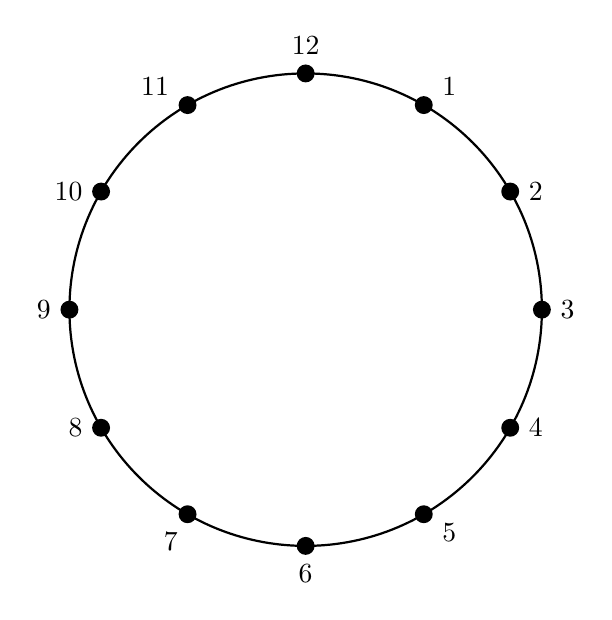
\begin{tikzpicture}
[nodedecorate/.style={shape=circle,inner sep=2pt,draw,thick,fill=black},%
  linedecorate/.style={-,thick},%
  scale=3]
\draw [thick] (0,0) circle (1cm);
%% nodes or vertices
\foreach \nodename/\x/\y/\direction/\navigate in {
  1/0.5/0.866/above right/east, 2/0.866/0.5/right/east,
  3/1/0/right/east, 4/0.866/-0.5/right/east,
  5/0.5/-0.866/below right/east, 6/0/-1/below/south,
  7/-0.5/-0.866/below left/south, 8/-0.866/-0.5/left/west,
  9/-1/0/left/west, 10/-0.866/0.5/left/west,
  11/-0.5/0.866/above left/west, 12/0/1/above/north}
{
  \node (\nodename) at (\x,\y) [nodedecorate] {};
  \node [\direction] at (\nodename.\navigate) {$\nodename$};
}
\end{tikzpicture}
\caption{A $12$-hour clock face\index{clock face}.}
\label{fig:number_theory:12_hour_clock_face}
\end{figure}

The command \verb!mod!\index{$\bmod$} allows us to compute such a
remainder.

\begin{lstlisting}
sage: mod(23, 5)
3
sage: mod(8, 5)
3
sage: mod(1, 12)
1
sage: mod(2, 12)
2
sage: mod(13, 12)
1
sage: mod(14, 12)
2
\end{lstlisting}

If \verb!n! is an integer, we could also use \verb!n.quo_rem(m)! to
obtain the quotient\index{quotient} and remainder\index{remainder}
upon dividing \verb!n! by \verb!m!. The output of \verb!n.quo_rem(m)!
is a tuple consisting of two integers. The first integer is the
quotient and the second is the remainder.
%
\begin{lstlisting}
sage: 1.quo_rem(12)
(0, 1)
sage: q, r = 14.quo_rem(12)
sage: q; r
1
2
sage: r == Integer(mod(14, 12))
True
sage: r == mod(14, 12).lift()
True
sage: r; mod(14, 12)
2
2
\end{lstlisting}
%
In the last code listing, we first converted \verb!mod(14, 12)! to an
integer using \verb!Integer!. The result is then compared with the
remainder \verb!r!. We could also use \verb!mod(14, 12).lift()! to
convert the output of \verb!mod(14, 12)! to an integer prior to
comparing with \verb!r!.


%%%%%%%%%%%%%%%%%%%%%%%%%%%%%%%%%%%%%%%%%%%%%%%%%%%%%%%%%%%%%%%%%%%%%%%%%%%

\section{Kid RSA}
\index{cryptography}
\index{Kid RSA}

This section presents Kid RSA~\cite[p.17]{Koblitz1998}, a simplified
version of the RSA\index{RSA} cryptosystem. Neal
Koblitz\index{Koblitz, Neal} developed Kid RSA\index{Kid RSA} as a
tool for teaching cryptography without requiring advanced
mathematics. Most of the necessary concepts and techniques for
understanding Kid RSA are already presented in this chapter. It is
very important to point out that this section is \emph{not} an
introduction to cryptography. Materials presented in this section are
intended for teaching and learning purposes only. If you require more
details about cryptography, please consult specialized texts such
as~\cite{MenezesEtAl1996,Stinson2006,TrappeWashington2006}.

In the Kid RSA system, there are two keys: the
\emph{public key}\index{public key} and its corresponding
\emph{private key}\index{private key}. A public key is used for
\emph{scrambling} messages that you want to keep secret from prying
eyes. The private key corresponding to your public key is used for
\emph{unscrambling} the gibberish resulting from the scrambling
process. In principle, only your private key can unscramble the
gibberish that has been scrambled using your public key. You can let
anyone know your public key. But you should keep your private key only
to yourself. (You don't want anyone to read that scrambled love
letter, right?)

Here is how Kid RSA works. First, Alice chooses four random positive
integers $a, b, A, B$ and computes the following numbers:
%
\begin{align*}
M &= ab - 1 \\[4pt]
e &= AM + a \\[4pt]
d &= BM + b \\[4pt]
n &= \frac{ed - 1}{M}.
\end{align*}
%
Her public key is the pair $(n, e)$ and her private key is $d$.

A message in Kid RSA is any positive integer $x < n$. Alice's friend,
Bob, wants to send her a secret message $x$. Using Alice's public key,
Bob scrambles the message $x$ by multiplying $x$ by $e$, then dividing
the product $xe$ by $n$. The remainder $y$ upon dividing $xe$ by $n$
is the scrambled message. Bob can now send $y$~(the scrambled message)
to Alice via email, the postal service, etc.

To unscramble $y$, Alice multiplies $y$ by her private key $d$ to
obtain the product $yd$. She then divides $yd$ by $n$ and keeps only
the remainder resulting from this division. The remainder upon
dividing $yd$ by $n$ is Bob's original unscrambled message $x$.

As an example, suppose Alice chooses the positive integers
\[
a = 4,\quad
b = 5,\quad
A = 6,\quad
B = 7.
\]
%
\begin{lstlisting}
sage: a = 4; b = 5; A = 6; B = 7
sage: M = a*b - 1
sage: e = A*M + a
sage: d = B*M + b
sage: n = (e*d - 1) / M
sage: n, e
(857, 118)
sage: d
138
\end{lstlisting}
%
Then her public key is $(857, 118)$ and her private key is $138$. Bob
wants to send Alice the message $x = 500$. What is the scrambled
version of $x$?
%
\begin{lstlisting}
sage: x = 500
sage: y = Integer(mod(x*e, n)); y
724
\end{lstlisting}
%
The scrambled version of $x$ is $y = 724$. Bob can now send $y = 724$
to Alice. To unscramble $y = 724$, Alice performs the following
computation:
%
\begin{lstlisting}
sage: mod(y*d, n)
500
sage: x
500
sage: Integer(mod(y*d, n)) == x
True
\end{lstlisting}
%
Thus Bob's original message is successfully unscrambled.


%%%%%%%%%%%%%%%%%%%%%%%%%%%%%%%%%%%%%%%%%%%%%%%%%%%%%%%%%%%%%%%%%%%%%%%%%%%

\section*{Problems}
\addcontentsline{toc}{section}{Problems}

\begin{enumerate}
\item For the function $f(x) = x^2 + x + 41$, restrict $x$ to take
  only nonnegative integer values.
  \begin{enumerate}
  \item Which integer values of $x$ would result in $f(x)$ being a
    prime number?

  \item What is the largest integer $x$ such that $f(x)$ is prime?

  \item What is the smallest nonnegative integer $x$ such that $f(x)$
    is not prime?
  \end{enumerate}
\end{enumerate}

%%%%%%%%%%%%%%%%%%%%%%%%%%%%%%%%%%%%%%%%%%%%%%%%%%%%%%%%%%%%%%%%%%%%%%%%%%%

\chapter{Linear Functions}

\begin{enumerate}
\item Linear equations and inequalities

\item Graphs of linear equations and inequalities:
  \begin{enumerate}
  \item gradients of linear equations

  \item formulas for linear equations
  \end{enumerate}

\item Solving linear equations and inequalities

\item Simultaneous equations

\item Parallel and perpendicular lines

\item Midpoint and intersection of two lines

\item Distance between two points

\item Fitting linear functions to data
\end{enumerate}


%%%%%%%%%%%%%%%%%%%%%%%%%%%%%%%%%%%%%%%%%%%%%%%%%%%%%%%%%%%%%%%%%%%%%%%%%%%

\section{Linear equations and inequalities}

A \emph{linear equation} is an expression of the form
%
\begin{equation}
\label{eq:linear_functions:linear_equation_general_form}
y
=
ax + b
\end{equation}
%
where $a$ and $b$ can be any real numbers. Allowing $a$ to be zero
would result in $y = 0 \times x + b = b$, whose graph is a horizontal
line through the number $b$ on the $y$-axis. The equation $y = b$
describes a horizontal line through the point $(0, b)$, as illustrated
in Figure~\ref{fig:linear_functions:horizontal_line}. If $b = 0$ but
$a \neq 0$, then the linear
equation~(\ref{eq:linear_functions:linear_equation_general_form})
simplifies to $y = ax$. We can visualize this equation as a line
through the origin, as shown in
Figure~\ref{fig:linear_functions:line_through_origin}.

\begin{figure}[!htbp]
\centering
%% graph of horizontal line
\subfigure[$y = b$]{
\label{fig:linear_functions:horizontal_line}
\begin{tikzpicture}
[linestyle/.style={semithick},%
 axisstyle/.style={semithick,->,>=stealth}]
%% graph of function
\draw[linestyle] (-2,2) -- (4,2);
\draw[fill] (0,2) circle (0.08cm) node[above left]{$(0,b)$};
%% horizontal and vertical axes
\draw[axisstyle] (-2,0) -- (4,0) node[right]{$x$};
\draw[axisstyle] (0,-0.5) -- (0,3) node[above]{$y$};
\end{tikzpicture}
}
\quad
%%
%% graph of line through the origin
\subfigure[$y = ax$]
{\label{fig:linear_functions:line_through_origin}
\begin{tikzpicture}
[linestyle/.style={semithick},%
 axisstyle/.style={semithick,->,>=stealth},%
 domain=-0.25:1.5]
%% graph of function
\draw[linestyle] plot (\x, {2*\x});
%% horizontal and vertical axes
\draw[axisstyle] (-2,0) -- (4,0) node[right]{$x$};
\draw[axisstyle] (0,-0.5) -- (0,3) node[above]{$y$};
\end{tikzpicture}
}
\caption{Plot of the horizontal line and line through the origin.}
\end{figure}

In the equation $y = ax + b$, the factor $a$ is called the
\emph{gradient} and $b$ is the $y$-intercept. Given the equation
%
\begin{equation}
\label{eq:linear_functions:example_linear_equation}
y
=
3x + 5
\end{equation}
%
we can tell that the gradient is $a = 3$ and the $y$-intercept is
$b = 5$. The coordinate of the $y$-intercept is $(0, 5)$. Another way
to derive this coordinate is to set $x = 0$
in~(\ref{eq:linear_functions:example_linear_equation}) and solve the
resulting equation for $y$. That is,
\[
y
=
3 \times 0 + 5
=
5
\]
In other words, the $y$-intercept
of~(\ref{eq:linear_functions:example_linear_equation}) is the point
where $x = 0$ and $y = 5$. To find the $x$-intercept
of~(\ref{eq:linear_functions:example_linear_equation}), we set $y = 0$
in~(\ref{eq:linear_functions:example_linear_equation}) and solve the
resulting equation $0 = 3x + 5$ for $x$ to get $x = -5 / 3$. Thus the
$x$-intercept is $-5/3$, and the coordinate of the $x$-intercept is
$(0,\; -5/3)$.

\begin{lstlisting}
sage: var("x, y");
sage: solve(y == 0*x + 5, y)
[y == 5]
sage: solve(0 == 3*x + 5, x)
[x == (-5/3)]
\end{lstlisting}

A \emph{linear inequality} has the general form as a linear equation,
but the equal sign is now replaced by the inequality sign:
\[
y
\leq
ax + b.
\]

%%%%%%%%%%%%%%%%%%%%%%%%%%%%%%%%%%%%%%%%%%%%%%%%%%%%%%%%%%%%%%%%%%%%%%%%%%%
%% This file is part of the book
%%
%% Sage for High School
%% http://code.google.com/p/high-school-sage/
%%
%% Copyright (C) 2010 Minh Van Nguyen <nguyenminh2@gmail.com>
%%
%% See the file COPYING for copying conditions. See the file LICENSE
%% for the terms under which the whole book is licensed.
%%%%%%%%%%%%%%%%%%%%%%%%%%%%%%%%%%%%%%%%%%%%%%%%%%%%%%%%%%%%%%%%%%%%%%%%%%%

\chapter{Quadratic Functions}

\begin{enumerate}
\item Solving quadratic equations:
  \begin{enumerate}
  \item rational solutions

  \item real solutions

  \item the quadratic formula
  \end{enumerate}

\item The discriminant

\item Graphs of quadratic equations

\item Approximate location of roots

\item Solving quadratic equations by iteration

\item Simultaneous equations: linear and quadratic
\end{enumerate}

%%%%%%%%%%%%%%%%%%%%%%%%%%%%%%%%%%%%%%%%%%%%%%%%%%%%%%%%%%%%%%%%%%%%%%%%%%%

\chapter{Polynomials and Their Factorization}

\begin{enumerate}
\item Polynomials:
  \begin{enumerate}
  \item Evaluating polynomials

  \item Adding, subtracting, multiplying, and dividing polynomials
  \end{enumerate}

\item Factors and common factors

\item Factorizing using the distributive laws:
  \begin{enumerate}
  \item binomial expansion

  \item difference of two squares

  \item perfect squares

  \item completing the squares
  \end{enumerate}

\item Factorizing four terms:
  \begin{enumerate}
  \item Grouping two and two

  \item Grouping three and one
  \end{enumerate}

\item Long division

\item The remainder theorem

\item The factor theorem
\end{enumerate}

%%%%%%%%%%%%%%%%%%%%%%%%%%%%%%%%%%%%%%%%%%%%%%%%%%%%%%%%%%%%%%%%%%%%%%%%%%%
%% This file is part of the book
%%
%% Sage for High School
%% http://code.google.com/p/high-school-sage/
%%
%% Copyright (C) 2010 Minh Van Nguyen <nguyenminh2@gmail.com>
%%
%% See the file COPYING for copying conditions. See the file LICENSE
%% for the terms under which the whole book is licensed.
%%%%%%%%%%%%%%%%%%%%%%%%%%%%%%%%%%%%%%%%%%%%%%%%%%%%%%%%%%%%%%%%%%%%%%%%%%%

\chapter{Exponential and Logarithmic Functions}

\begin{enumerate}
\item The family of exponential functions

\item Comparing exponential and linear functions

\item Graphs of exponential functions

\item Continuous growth

\item Properties of logarithms

\item Logarithms and exponential functions

\item The logarithmic function

\item Logarithmic scales
\end{enumerate}

%%%%%%%%%%%%%%%%%%%%%%%%%%%%%%%%%%%%%%%%%%%%%%%%%%%%%%%%%%%%%%%%%%%%%%%%%%%

\chapter{Transformations of Functions}

\begin{enumerate}
\item Vertical and horizontal shifts

\item Reflections and symmetry

\item Vertical stretches and compressions

\item Horizontal stretches and compressions
\end{enumerate}

%%%%%%%%%%%%%%%%%%%%%%%%%%%%%%%%%%%%%%%%%%%%%%%%%%%%%%%%%%%%%%%%%%%%%%%%%%%

\chapter{Trigonometic Functions}

\begin{enumerate}
\item The sine and cosine functions

\item Degrees and radians

\item Graphing the sine and cosine functions

\item Sinusoidal functions

\item More trigonometric functions

\item Inverse trigonometric functions

\item Trigonometric simplification:
  \begin{enumerate}
  \item trigonometric identities

  \item sum and difference formulas for sine and cosine
  \end{enumerate}
\end{enumerate}

%%%%%%%%%%%%%%%%%%%%%%%%%%%%%%%%%%%%%%%%%%%%%%%%%%%%%%%%%%%%%%%%%%%%%%%%%%%

\chapter{Vectors and Matrices}


%%%%%%%%%%%%%%%%%%%%%%%%%%%%%%%%%%%%%%%%%%%%%%%%%%%%%%%%%%%%%%%%%%%%%%%%%%%

\section{Scalars and vectors}
\label{sec:scalars_vectors}

The path of a car travelling from location $A$ to location $B$ is
characterized by two quantities or \emph{scalars}\index{scalars}: a
magnitude\index{magnitude}~(such as speed), and a direction~(from $A$
to $B$). Both of these two scalars are summarized by a
\emph{vector}\index{vector}.

\begin{figure}[!htpb]
\centering
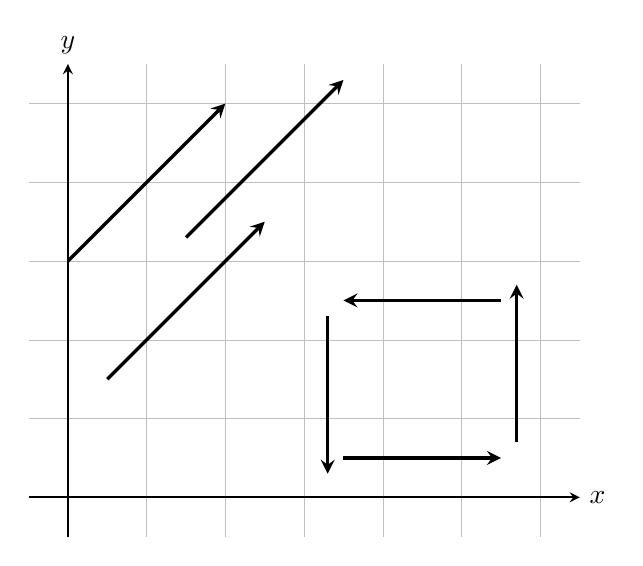
\begin{tikzpicture}
[linedecorate/.style={->,>=stealth,very thick}]
% grids for the plane
\draw[step=1cm,lightgray,very thin] (-0.5,-0.5) grid (6.5,5.5);
% the rectangular axes
\draw[->,>=stealth,semithick] (-0.5,0) -- (6.5,0) node[right]{$x$};
\draw[->,>=stealth,semithick] (0,-0.5) -- (0,5.5) node[above]{$y$};
% vectors
\draw[linedecorate] (0,3) -- node[above left]{$\vecu$} (2,5);
\draw[linedecorate] (1.5,3.3) -- node[below right]{$\vecv$} (3.5,5.3);
\draw[linedecorate] (0.5,1.5) -- node[below right]{$\vecw$} (2.5,3.5);
\draw[linedecorate] (3.5,0.5) -- (5.5,0.5);
\draw[linedecorate] (5.7,0.7) -- (5.7,2.7);
\draw[linedecorate] (5.5,2.5) -- (3.5,2.5);
\draw[linedecorate] (3.3,2.3) -- (3.3,0.3);
\end{tikzpicture}
\caption{Vectors in the $x$-$y$ plane.}
\label{fig:vectors_matrices:plane_vectors}
\end{figure}

In the $x$-$y$ plane, we can visualize a vector as an arrow from point
$A$ to point $B$~(see
Figure~\ref{fig:vectors_matrices:plane_vectors}). The starting point
$A$ of the vector is called the \emph{tail}\index{vectors!tail} and
the terminal point $B$ is the \emph{head}.\index{vectors!head} Two
vectors are \emph{equivalent}\index{vectors!equivalent} if they have
the same magnitude and direction. The vectors $\vecu$, $\vecv$, and
$\vecw$ in Figure~\ref{fig:vectors_matrices:plane_vectors} are thus
all equivalent to each other.

To analyze vectors using algebra, we can think of a vector $\vecu$
as starting from the origin of the $x$-$y$ plane and having
$(u_1, u_2)$ as the coordinate for its head~(see
Figure~\ref{fig:specify_vector_head_coordinate}). So $\vecu$ is
completely determined by the coordinate of its head and we write
$\vecu = \langle u_1, u_2 \rangle$ as an algebraic representation
for $\vecu$.

\begin{figure}[!htpb]
\centering
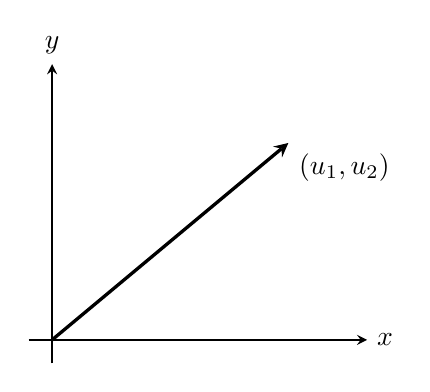
\begin{tikzpicture}
% the rectangular axes
\draw[->,>=stealth,semithick] (-0.3,0) -- (4,0) node[right]{$x$};
\draw[->,>=stealth,semithick] (0,-0.3) -- (0,3.5) node[above]{$y$};
% vector described by its head coordinate
\draw[->,>=stealth,very thick] (0,0) -- node[above left]{$\vecu$} (3,2.5) node[below right]{$(u_1, u_2)$};
\end{tikzpicture}
\caption{A vector as specified by its head coordinate.}
\label{fig:specify_vector_head_coordinate}
\end{figure}

In case the tail of $\vecu$ is not the origin, we let $(x_1, y_1)$
be the coordinate of the tail and denote the coordinate of the head by
$(x_2, y_2)$. By subtracting coordinatewise, we obtain an equivalent
vector $\vecv$ that emanates from the origin of the $x$-$y$
plane. The coordinate of $\vecv$ is
\[
(x_2, y_2) - (x_1, y_1)
=
(x_2 - x_1,\; y_2 - y_1)
=
(u_1, u_2)
\]
and we do not distinguish between $\vecu$ and $\vecv$. Thus we
can transform $\vecu$ to be a vector emanating from the origin and
specified by the coordinate
%
\begin{equation}
\label{eq:component_form_vector}
\vecu
=
\langle x_2 - x_1,\; y_2 - y_1 \rangle
=
\langle u_1, u_2 \rangle.
\end{equation}
%
Equation~(\ref{eq:component_form_vector}) is called the
\emph{component form}\index{component form} of a vector, with $u_1$
and $u_2$ being the individual components. The vector
$\veczero = \langle 0, 0 \rangle$ is called the zero
vector.\index{zero vector}

\begin{figure}[!htpb]
\centering
\begin{tikzpicture}
% the rectangular axes
\draw[->,>=stealth,semithick] (-2.5,0) -- (5.7,0) node[right]{$x$};
\draw[->,>=stealth,semithick] (0,-1.5) -- (0,6.7) node[above]{$y$};
% ticks on horizontal axis
\foreach \x in {-2,-1,-1}
  \draw (\x cm,2pt) -- (\x cm,-2pt) node[anchor=north] {$\x$};
\foreach \x in {1,2,...,5}
  \draw (\x cm,2pt) -- (\x cm,-2pt) node[anchor=north] {$\x$};
% ticks on vertical axis
\foreach \y in {-1,-1}
  \draw (2pt,\y cm) -- (-2pt,\y cm) node[anchor=east] {$\y$};
\foreach \y in {1,2,...,6}
  \draw (2pt,\y cm) -- (-2pt,\y cm) node[anchor=east] {$\y$};
% vector u
\draw[->,>=stealth,very thick] (-2,-1) node[below]{$(-2,-1)$} -- node[above left]{$\vecu$} (1,3) node[above]{$(1,3)$};
% vector v
\draw[->,>=stealth,very thick] (1.5,1.5) node[below]{$(1.5,1.5)$} -- node[above left]{$\vecv$} (4.5,5.5) node[above]{$(4.5,5.5)$};
\end{tikzpicture}
\caption{Verify that vectors $\vecu$ and $\vecv$ are equivalent.}
\label{fig:vectors_matrices:verify_vectors_u_v}
\end{figure}

\begin{example}
Let the vector $\vecu$ be described by the directed line segment
from $(-2,-1)$ to $(1,3)$, and let $\vecv$ be the line segment from
$(1.5,1.5)$ to $(4.5,5.5)$, as shown in
Figure~\ref{fig:vectors_matrices:verify_vectors_u_v}. Show that
$\vecu$ and $\vecv$ are equivalent vectors.
\end{example}

\begin{proof}[Solution]
To show that $\vecu$ and $\vecv$ are equivalent, we need to show
that they have the same length and are in the same direction. The
length of $\vecu$ is equivalent to the length of the line segment
from $(-2,-1)$ to $(1,3)$:
%
\begin{align*}
\sqrt{(1 - (-2))^2 + (3 - (-1))^2}
&=
\sqrt{(1 + 2)^2 + (3 + 1)^2} \\
&=
\sqrt{9 + 16} \\
&=
5.
\end{align*}
%
This tells us that $\vecu$ has length 5. Similarly, the length of
$\vecv$ is
%
\begin{align*}
\sqrt{(4.5 - 1.5)^2 + (5.5 - 1.5)^2}
&=
\sqrt{3^2 + 4^2} \\
&=
\sqrt{9 + 16} \\
&=
5
\end{align*}
%
which is the same length as that of $\vecu$.

\begin{lstlisting}
sage: u = vector([1 - (-2), 3 - (-1)]); u
(3, 4)
sage: v = vector([4.5 - 1.5, 5.5 - 1.5]); v
(3.000...000, 4.000...000)
sage: u.norm()
5
sage: v.norm()
5.000...000
\end{lstlisting}

The slope of the line segment from $(-2,-1)$ to $(1,3)$ is
\[
\frac{3 - (-1)} {1 - (-2)}
=
\frac{4}{3}
\]
and the slope of the line segment from $(1.5,1.5)$ to $(4.5,5.5)$ is
\[
\frac{5.5 - 1.5}{4.5 - 1.5}
=
\frac{4}{3}
\]
which shows that these two line segments have the same direction, so
$\vecu$ and $\vecv$ point in the same direction.
%
\begin{lstlisting}
sage: (3 - (-1)) / (1 - (-2))
4/3
sage: (5.5 - 1.5) / (4.5 - 1.5)
1.333...333
sage: QQ((5.5 - 1.5) / (4.5 - 1.5))
4/3
\end{lstlisting}
%
Therefore, $\vecu$ and $\vecv$ are equivalent vectors.
\end{proof}

We denote the length of a vector as follows. Let $\vecu$ be a
vector whose starting point is $P = (x_1, y_1)$ and whose terminal
point is $Q = (x_2, y_2)$. Then the length or magnitude of $\vecu$
is denoted by $\vecvertl \vecu \vecvertr$ and given
by the equation
%
\begin{equation}
\label{eq:vectors_matrices:magnitude_two_dimensional_vector}
\begin{aligned}
\vecvertl \vecu \vecvertr
&=
\sqrt{(x_2 - x_1)^2 + (y_2 - y_1)^2} \\
&=
\sqrt{v_1^2 + v_2^2}.
\end{aligned}
\end{equation}


%%%%%%%%%%%%%%%%%%%%%%%%%%%%%%%%%%%%%%%%%%%%%%%%%%%%%%%%%%%%%%%%%%%%%%%%%%%

\section{Add, subtract, and multiply vectors}
\index{vectors!arithmetic}
%% Relate vectors with complex numbers.

The left-hand side of Figure~\ref{fig:vectors_matrices:vector_sum}
illustrates the path of an object. Initially travelling in the
direction of vector $\vecu$, the object then changes its direction to
move in the direction of $\vecv$. The total displacement of the object
is represented as the vector $\vecu + \vecv = \vecw$. Furthermore, we
could first go in the direction of $\vecv$ and then in that of $\vecu$,
and hence obtain the same displacement $\vecv + \vecu = \vecw$, as
shown on the right-hand side of
Figure~\ref{fig:vectors_matrices:vector_sum}. This ``adding'' of
vectors is just one of many basic operations that can be performed on
vectors. In fact, the ``adding'' rule illustrated in
Figure~\ref{fig:vectors_matrices:vector_sum} is called the
\emph{parallelogram rule}\index{parallelogram rule} for vector
addition.

\begin{figure}[!htpb]
\centering
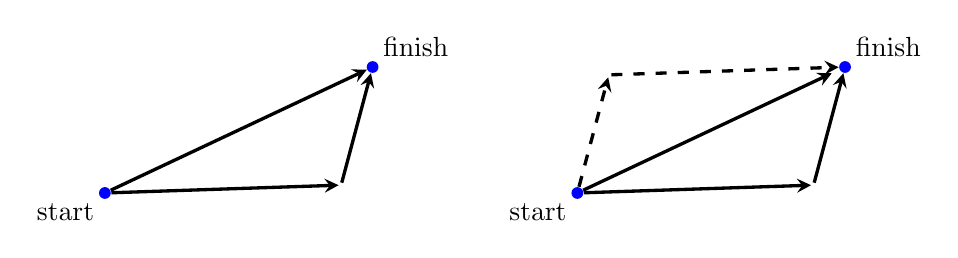
\begin{tikzpicture}
% left set of vectors
\node (start1) at (0,0) [circle,fill=blue,inner sep=1.5pt]{};
\node (middle1) at (3,0.1) [circle,inner sep=0.5pt]{};
\node (finish1) at (3.4,1.6) [circle,fill=blue,inner sep=1.5pt]{};
\draw[->,>=stealth,very thick] (start1) node[below left]{start}  -- node[below]{$\vecu$} (middle1);
\draw[->,>=stealth,very thick] (middle1) -- node[right]{$\vecv$} (finish1) node[above right]{finish};
\draw[->,>=stealth,very thick] (start1) -- node[above]{$\vecw$} (finish1);
% right set of vectors
\node (start2) at (6,0) [circle,fill=blue,inner sep=1.5pt]{};
\node (lowerMiddle) at (9,0.1) [circle,inner sep=0.5pt]{};
\node (upperMiddle) at (6.4,1.5) [circle,inner sep=0.5pt]{};
\node (finish2) at (9.4,1.6) [circle,fill=blue,inner sep=1.5pt]{};
\draw[->,>=stealth,very thick] (start2) node[below left]{start} -- node[below]{$\vecu$} (lowerMiddle);
\draw[->,>=stealth,very thick] (lowerMiddle) -- node[right]{$\vecv$} (finish2) node[above right]{finish};
\draw[->,>=stealth,shorten >=3pt,very thick] (start2) -- node[above]{$\vecw$} (finish2);
\draw[->,>=stealth,very thick,dash pattern=on 4pt off 4pt] (start2) -- node[left]{$\vecv$} (upperMiddle);
\draw[->,>=stealth,very thick,dash pattern=on 4pt off 4pt] (upperMiddle) -- node[above]{$\vecu$} (finish2);
\end{tikzpicture}
\caption{The vector sum $\vecu + \vecv = \vecw = \vecv + \vecu$.}
\label{fig:vectors_matrices:vector_sum}
\end{figure}

\begin{definition}
\label{def:vectors_matrices:vector_operations}
Let $\vecu = \langle u_1, u_2 \rangle$ and
$\vecv = \langle v_1, v_2 \rangle$ be vectors and suppose
$c$ is a scalar. Then we have the following operations on vectors:
\begin{enumerate}
\item The \emph{vector sum} of $\vecu$ and
  $\vecv$ is $\vecu + \vecv = \langle u_1 + v_1,\; u_2 + v_2 \rangle$.

\item The \emph{negative} of $\vecu$ is
  $-\vecu = \langle -u_1, -u_2 \rangle$.

\item The \emph{vector difference} of $\vecu$ and
  $\vecv$ is $\vecu - \vecv =
  \langle u_1, u_2 \rangle - \langle v_1, v_2 \rangle = \langle u_1 -
  v_1,\; u_2 - v_2 \rangle$.

\item The \emph{scalar multiple} of $c$ and $\vecu$ is
  $c\vecu = \langle c u_1, c u_2 \rangle$.
\end{enumerate}
\end{definition}

The negative of a vector $\vecu$ is a vector that has the same
length as $\vecu$, but goes in the opposite direction. One
exception is the zero vector $\veczero$, whose negative is itself
because $-\veczero = -\langle 0,0 \rangle = \langle -0, -0 \rangle =
\langle 0,0 \rangle = \veczero$. More generally, scalar
multiplication has the effect of scaling a vector. This may result in
expanding the vector, contracting it, producing the negative of the
vector, or expanding/contracting the negative of the vector. These
various possibilities are shown in
Figure~\ref{fig:scalar_multiply_negative}.

\begin{figure}[!htpb]
\centering
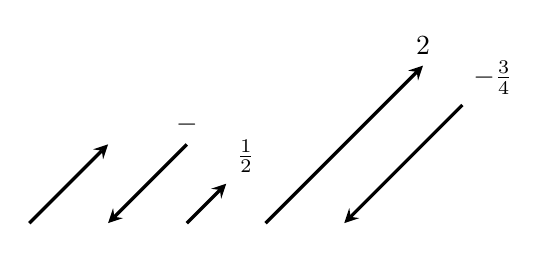
\begin{tikzpicture}
\draw[->,>=stealth,very thick] (0,0) -- (1,1) node[above]{$\vecu$};
\draw[<-,>=stealth,very thick] (1,0) -- (2,1) node[above]{$-\vecu$};
\draw[->,>=stealth,very thick] (2,0) -- (2.5,0.5) node[above right]{$\frac{1}{2}\vecu$};
\draw[->,>=stealth,very thick] (3,0) -- (5,2) node[above]{$2\vecu$};
\draw[<-,>=stealth,very thick] (4,0) -- (5.5,1.5) node[above right]{$-\frac{3}{4}\vecu$};
\end{tikzpicture}
\caption{Scalar multiplication and negative of a vector.}
\label{fig:scalar_multiply_negative}
\end{figure}

Using the parallelogram rule for vector addition, we can similarly
illustrate vector difference. The left-hand side of
Figure~\ref{fig:vectors_matrices:vector_difference_parallelogram_triangle} shows the
parallelogram rule for vector subtraction, while the right-hand side shows
the triangle rule for vector subtraction. Thus to determine the
difference of two vectors $\vecu$ and $\vecv$, we first align the
vectors so that their initial points coincide. Then the difference
$\vecu - \vecv$ is the vector that starts from the head of
$\vecv$ and ends at the terminal point of $\vecu$.

\begin{figure}[!htpb]
\centering
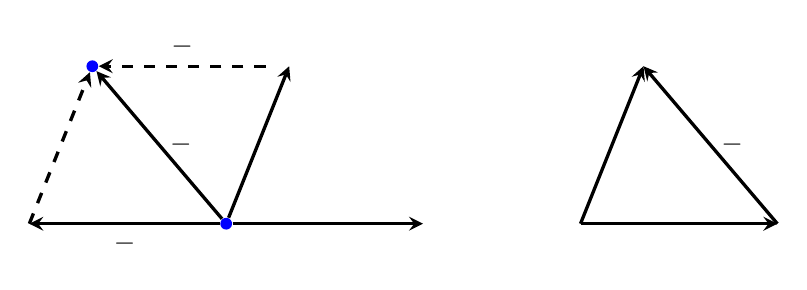
\begin{tikzpicture}
% left-hand figure: vector difference by parallelogram rule
\node (origin) at (0,0) [circle,fill=blue,inner sep=1.5pt]{};
\node (destin) at (-1.7,2) [circle,fill=blue,inner sep=1.5pt]{};
\draw[->,>=stealth,very thick] (origin) -- node[below]{$\vecv$} (2.5,0);
\draw[->,>=stealth,very thick] (origin) -- node[below]{$-\vecv$} (-2.5,0);
\draw[->,>=stealth,very thick] (origin) -- node[right]{$\vecu$} (0.8,2);
\draw[->,>=stealth,very thick,dash pattern=on 4pt off 4pt] (-2.5,0) -- node[left]{$\vecu$} (destin);
\draw[->,>=stealth,very thick,dash pattern=on 4pt off 4pt] (0.5,2) -- node[above]{$-\vecv$} (destin);
\draw[->,>=stealth,very thick] (origin) -- node[right]{$\vecu - \vecv$} (destin);
% right-hand figure: vector difference
\draw[->,>=stealth,very thick] (4.5,0) -- node[left]{$\vecu$} (5.3,2);
\draw[->,>=stealth,very thick] (4.5,0) -- node[below]{$\vecv$} (7,0);
\draw[->,>=stealth,very thick] (7,0) -- node[right]{$\vecu - \vecv$} (5.3,2);
\end{tikzpicture}
\caption{Vector difference by the parallelogram rule~(left) and by the
triangle rule~(right).}
\label{fig:vectors_matrices:vector_difference_parallelogram_triangle}
\end{figure}

Vector operations share many of the familiar properties of operations
on real numbers. Given two real numbers, for example, it does not
matter in which order we add
them. Problem~\ref{prob:vectors_matrices:field_laws_for_vectors} lists
a number of vector rules that are similar to those obeyed by real numbers.

\begin{example}
Using vector rules from
problem~\ref{prob:vectors_matrices:field_laws_for_vectors}, find a
vector $\vecx$ such that $5\vecx + 7\vecu = 4\vecv$.
\end{example}

\begin{proof}[Solution]
First, subtract $7\vecu$ from both sides of the equal sign to get
$5\vecx + (7\vecu - 7\vecu) = 4\vecv - 7\vecu$, which can be
simplified to $5\vecx = 4\vecv - 7\vecu$. Now divide both sides of
the last equation by $5$ and we have
$\frac{1}{5} (5\vecx) = \frac{1}{5} (4\vecv - 7\vecu)$. Simplify the
last equation to
$\vecx = \frac{1}{5} (4\vecv) + \frac{1}{5}(-7\vecu)$. So the required
vector is $\vecx = \frac{4}{5}\vecv - \frac{7}{5}\vecu$.
\end{proof}

Any nonzero vector $\vecv$ can be transformed into a vector $\vecu$ of
magnitude $1$. The equation to effect this transformation is
%
\begin{equation}
\label{eq:vectors_matrices:two_dimensional_unit_vector}
\vecu
=
\frac {\vecv} {\vecvertl \vecv \vecvertr}
=
\vecv
\frac {1} {\vecvertl \vecv \vecvertr}.
\end{equation}
%
The process of using
equation~(\ref{eq:vectors_matrices:two_dimensional_unit_vector}) to
transform a nonzero vector into a vector of magnitude $1$ is called
\emph{normalizing}\index{vectors!normalization} a vector. For example,
given the vector $\vecu = \langle 1, 2 \rangle$, we can use
equation~(\ref{eq:vectors_matrices:two_dimensional_unit_vector}) to
find the normalized form of $\vecu$. Since
$\vecvertl \vecu \vecvertr = \sqrt{5}$ by
equation~(\ref{eq:vectors_matrices:magnitude_two_dimensional_vector}),
so $\vecu$ is normalized as
%
\begin{align*}
\frac {\vecu} {\vecvertl \vecu \vecvertr}
&=
\frac{1}{\sqrt{5}} \langle 1, 2 \rangle \\[4pt]
&=
\frac{\sqrt{5}}{5} \langle 1, 2 \rangle.
\end{align*}

\begin{lstlisting}
sage: u = vector([1, 2])
sage: u / u.norm()
(1/5*sqrt(5), 2/5*sqrt(5))
\end{lstlisting}


%%%%%%%%%%%%%%%%%%%%%%%%%%%%%%%%%%%%%%%%%%%%%%%%%%%%%%%%%%%%%%%%%%%%%%%%%%%

\subsection{Applications to geometry}
\label{subsec:2D_vectors_apply_geometry}

A line in the $x$-$y$ plane is usually described by the linear
equation
\[
y = mx + c
\]
where $m \neq 0$ is the slope of the line and $c$ is a constant. The
same line can be represented in \emph{vector form}\index{vector form}
as
%
\begin{equation}
\label{eq:vector_form_line}
\langle x,\, mx + c \rangle
=
\langle 0, c \rangle + x \langle 1, m \rangle.
\end{equation}
%
The vector $\langle 0, c \rangle$ points to the line, while the vector
$\langle 1, m \rangle$ is in the same direction as the line.

\begin{example}
Express the line $2x + 3y = 4$ in vector form.
\end{example}

\begin{proof}[Solution]
Solving the equation $2x + 3y = 4$ for $y$ to get
\[
y = \frac{4}{3} - \frac{2}{3} x.
\]
Using equation~(\ref{eq:vector_form_line}), we have
\[
\langle 0,\, 4/3 \rangle
+ x \langle 1,\, -2/3 \rangle
\]
which is a representation of the line $2x + 3y = 4$ in vector form.
\end{proof}

In general, a line $L$ has many different vector representations. If
$(u_1, u_2)$ is a point on $L$, then $\vecu = \langle u_1, u_2
\rangle$ is a vector pointing to $L$. Furthermore, let $\vecv =
\langle v_1, v_2 \rangle$ be a vector in the same direction as
$L$. Then the line $L$ can be represented in vector form as
\[
\langle x, y \rangle
=
\vecu + t \vecv
\]
with $t$ being a parameter.

Two nonzero vectors $\vecu$ and $\vecv$ are said to be
\emph{linearly dependent}\index{linearly dependent} if they can be
expressed as a linear combination that equals the zero vector, i.e. we
can find two nonzero real numbers $m,n$ such that
$m\vecu + n\vecv = \veczero$. From this definition, it follows that
two vectors are parallel if and only if they are linearly
dependent. In other words, if two vectors are parallel then they are
linearly dependent. The converse is also true: if two vectors are
linearly dependent, then they are parallel.

%%%%%%%%%%%%%%%%%%%%%%%%%%%%%%%%%%%%%%%%%%%%%%%%%%%%%%%%%%%%%%%%%%%%%%%%%%%
%% This file is part of the book
%%
%% Sage for High School
%% http://code.google.com/p/high-school-sage/
%%
%% Copyright (C) 2010 Minh Van Nguyen <nguyenminh2@gmail.com>
%%
%% See the file COPYING for copying conditions. See the file LICENSE
%% for the terms under which the whole book is licensed.
%%%%%%%%%%%%%%%%%%%%%%%%%%%%%%%%%%%%%%%%%%%%%%%%%%%%%%%%%%%%%%%%%%%%%%%%%%%

\chapter{Polar Coordinates and Conic Sections}

\begin{enumerate}
\item Complex numbers and their algebra

\item Converting between polar and Cartesian coordinates
  \begin{enumerate}
  \item Polar form of complex numbers

  \item Multiplication and division using polar form

  \item De Moivre's theorem
  \end{enumerate}

\item Curves in polar coordinates

\item Conic sections:
  \begin{enumerate}
  \item circle

  \item ellipse

  \item parabola

  \item hyperbola
  \end{enumerate}
\end{enumerate}

%%%%%%%%%%%%%%%%%%%%%%%%%%%%%%%%%%%%%%%%%%%%%%%%%%%%%%%%%%%%%%%%%%%%%%%%%%%

\chapter{Statistics and Probability}

\begin{enumerate}
\item Mean, median, and mode

\item Plots:
  \begin{enumerate}
  \item Bar charts

  \item Histograms

  \item Stem-and-leaf plots

  \item Boxplot
  \end{enumerate}

\item Scatterplots:
  \begin{enumerate}
  \item $q$-correlation coefficient

  \item regression
  \end{enumerate}

\item Discrete probability distributions

\item Expectation and variance

\item Binomial distribution

\item Normal distribution
\end{enumerate}


%% appendices
\appendix
% This is set up to run with pdflatex.
%---------The file header---------------------------------------------
%% \documentclass[a4paper,12pt]{book}

%% \usepackage[english]{babel} %language selection
%% \selectlanguage{english}

%% \pagenumbering{arabic}

%% \usepackage{hyperref}
%% \hypersetup{colorlinks,
%%            citecolor=black,
%%            filecolor=black,
%%            linkcolor=black,
%%            urlcolor=black,
%%            bookmarksopen=true,
%%            pdftex}

%% \hfuzz = .6pt % avoid black boxes

%% \begin{document}
%---------------------------------------------------------------------
\chapter{GNU Free Documentation License}
%% \phantomsection  % so hyperref creates bookmarks
%% \addcontentsline{toc}{chapter}{GNU Free Documentation License}
%\label{label_fdl}

 \begin{center}

       Version 1.3, 3 November 2008


 Copyright \copyright{} 2000, 2001, 2002, 2007, 2008  Free Software Foundation, Inc.

 \bigskip

\url{http://www.fsf.org}

 \bigskip

 Everyone is permitted to copy and distribute verbatim copies
 of this license document, but changing it is not allowed.
\end{center}


\begin{center}
{\bf\large Preamble}
\end{center}

The purpose of this License is to make a manual, textbook, or other
functional and useful document ``free'' in the sense of freedom: to
assure everyone the effective freedom to copy and redistribute it,
with or without modifying it, either commercially or noncommercially.
Secondarily, this License preserves for the author and publisher a way
to get credit for their work, while not being considered responsible
for modifications made by others.

This License is a kind of ``copyleft'', which means that derivative
works of the document must themselves be free in the same sense.  It
complements the GNU General Public License, which is a copyleft
license designed for free software.

We have designed this License in order to use it for manuals for free
software, because free software needs free documentation: a free
program should come with manuals providing the same freedoms that the
software does.  But this License is not limited to software manuals;
it can be used for any textual work, regardless of subject matter or
whether it is published as a printed book.  We recommend this License
principally for works whose purpose is instruction or reference.


\begin{center}
{\Large\bf 1. APPLICABILITY AND DEFINITIONS\par}
%% \phantomsection
\addcontentsline{toc}{section}{1. APPLICABILITY AND DEFINITIONS}
\end{center}

This License applies to any manual or other work, in any medium, that
contains a notice placed by the copyright holder saying it can be
distributed under the terms of this License.  Such a notice grants a
world-wide, royalty-free license, unlimited in duration, to use that
work under the conditions stated herein.  The ``\textbf{Document}'', below,
refers to any such manual or work.  Any member of the public is a
licensee, and is addressed as ``\textbf{you}''.  You accept the license if you
copy, modify or distribute the work in a way requiring permission
under copyright law.

A ``\textbf{Modified Version}'' of the Document means any work containing the
Document or a portion of it, either copied verbatim, or with
modifications and/or translated into another language.

A ``\textbf{Secondary Section}'' is a named appendix or a front-matter section of
the Document that deals exclusively with the relationship of the
publishers or authors of the Document to the Document's overall subject
(or to related matters) and contains nothing that could fall directly
within that overall subject.  (Thus, if the Document is in part a
textbook of mathematics, a Secondary Section may not explain any
mathematics.)  The relationship could be a matter of historical
connection with the subject or with related matters, or of legal,
commercial, philosophical, ethical or political position regarding
them.

The ``\textbf{Invariant Sections}'' are certain Secondary Sections whose titles
are designated, as being those of Invariant Sections, in the notice
that says that the Document is released under this License.  If a
section does not fit the above definition of Secondary then it is not
allowed to be designated as Invariant.  The Document may contain zero
Invariant Sections.  If the Document does not identify any Invariant
Sections then there are none.

The ``\textbf{Cover Texts}'' are certain short passages of text that are listed,
as Front-Cover Texts or Back-Cover Texts, in the notice that says that
the Document is released under this License.  A Front-Cover Text may
be at most 5 words, and a Back-Cover Text may be at most 25 words.

A ``\textbf{Transparent}'' copy of the Document means a machine-readable copy,
represented in a format whose specification is available to the
general public, that is suitable for revising the document
straightforwardly with generic text editors or (for images composed of
pixels) generic paint programs or (for drawings) some widely available
drawing editor, and that is suitable for input to text formatters or
for automatic translation to a variety of formats suitable for input
to text formatters.  A copy made in an otherwise Transparent file
format whose markup, or absence of markup, has been arranged to thwart
or discourage subsequent modification by readers is not Transparent.
An image format is not Transparent if used for any substantial amount
of text.  A copy that is not ``Transparent'' is called ``\textbf{Opaque}''.

Examples of suitable formats for Transparent copies include plain
ASCII without markup, Texinfo input format, LaTeX input format, SGML
or XML using a publicly available DTD, and standard-conforming simple
HTML, PostScript or PDF designed for human modification.  Examples of
transparent image formats include PNG, XCF and JPG.  Opaque formats
include proprietary formats that can be read and edited only by
proprietary word processors, SGML or XML for which the DTD and/or
processing tools are not generally available, and the
machine-generated HTML, PostScript or PDF produced by some word
processors for output purposes only.

The ``\textbf{Title Page}'' means, for a printed book, the title page itself,
plus such following pages as are needed to hold, legibly, the material
this License requires to appear in the title page.  For works in
formats which do not have any title page as such, ``Title Page'' means
the text near the most prominent appearance of the work's title,
preceding the beginning of the body of the text.

The ``\textbf{publisher}'' means any person or entity that distributes
copies of the Document to the public.

A section ``\textbf{Entitled XYZ}'' means a named subunit of the Document whose
title either is precisely XYZ or contains XYZ in parentheses following
text that translates XYZ in another language.  (Here XYZ stands for a
specific section name mentioned below, such as ``\textbf{Acknowledgements}'',
``\textbf{Dedications}'', ``\textbf{Endorsements}'', or ``\textbf{History}''.)
To ``\textbf{Preserve the Title}''
of such a section when you modify the Document means that it remains a
section ``Entitled XYZ'' according to this definition.

The Document may include Warranty Disclaimers next to the notice which
states that this License applies to the Document.  These Warranty
Disclaimers are considered to be included by reference in this
License, but only as regards disclaiming warranties: any other
implication that these Warranty Disclaimers may have is void and has
no effect on the meaning of this License.


\begin{center}
{\Large\bf 2. VERBATIM COPYING\par}
%% \phantomsection
\addcontentsline{toc}{section}{2. VERBATIM COPYING}
\end{center}

You may copy and distribute the Document in any medium, either
commercially or noncommercially, provided that this License, the
copyright notices, and the license notice saying this License applies
to the Document are reproduced in all copies, and that you add no other
conditions whatsoever to those of this License.  You may not use
technical measures to obstruct or control the reading or further
copying of the copies you make or distribute.  However, you may accept
compensation in exchange for copies.  If you distribute a large enough
number of copies you must also follow the conditions in section~3.

You may also lend copies, under the same conditions stated above, and
you may publicly display copies.


\begin{center}
{\Large\bf 3. COPYING IN QUANTITY\par}
%% \phantomsection
\addcontentsline{toc}{section}{3. COPYING IN QUANTITY}
\end{center}


If you publish printed copies (or copies in media that commonly have
printed covers) of the Document, numbering more than 100, and the
Document's license notice requires Cover Texts, you must enclose the
copies in covers that carry, clearly and legibly, all these Cover
Texts: Front-Cover Texts on the front cover, and Back-Cover Texts on
the back cover.  Both covers must also clearly and legibly identify
you as the publisher of these copies.  The front cover must present
the full title with all words of the title equally prominent and
visible.  You may add other material on the covers in addition.
Copying with changes limited to the covers, as long as they preserve
the title of the Document and satisfy these conditions, can be treated
as verbatim copying in other respects.

If the required texts for either cover are too voluminous to fit
legibly, you should put the first ones listed (as many as fit
reasonably) on the actual cover, and continue the rest onto adjacent
pages.

If you publish or distribute Opaque copies of the Document numbering
more than 100, you must either include a machine-readable Transparent
copy along with each Opaque copy, or state in or with each Opaque copy
a computer-network location from which the general network-using
public has access to download using public-standard network protocols
a complete Transparent copy of the Document, free of added material.
If you use the latter option, you must take reasonably prudent steps,
when you begin distribution of Opaque copies in quantity, to ensure
that this Transparent copy will remain thus accessible at the stated
location until at least one year after the last time you distribute an
Opaque copy (directly or through your agents or retailers) of that
edition to the public.

It is requested, but not required, that you contact the authors of the
Document well before redistributing any large number of copies, to give
them a chance to provide you with an updated version of the Document.


\begin{center}
{\Large\bf 4. MODIFICATIONS\par}
%% \phantomsection
\addcontentsline{toc}{section}{4. MODIFICATIONS}
\end{center}

You may copy and distribute a Modified Version of the Document under
the conditions of sections 2 and 3 above, provided that you release
the Modified Version under precisely this License, with the Modified
Version filling the role of the Document, thus licensing distribution
and modification of the Modified Version to whoever possesses a copy
of it.  In addition, you must do these things in the Modified Version:

\begin{itemize}
\item[A.]
   Use in the Title Page (and on the covers, if any) a title distinct
   from that of the Document, and from those of previous versions
   (which should, if there were any, be listed in the History section
   of the Document).  You may use the same title as a previous version
   if the original publisher of that version gives permission.

\item[B.]
   List on the Title Page, as authors, one or more persons or entities
   responsible for authorship of the modifications in the Modified
   Version, together with at least five of the principal authors of the
   Document (all of its principal authors, if it has fewer than five),
   unless they release you from this requirement.

\item[C.]
   State on the Title page the name of the publisher of the
   Modified Version, as the publisher.

\item[D.]
   Preserve all the copyright notices of the Document.

\item[E.]
   Add an appropriate copyright notice for your modifications
   adjacent to the other copyright notices.

\item[F.]
   Include, immediately after the copyright notices, a license notice
   giving the public permission to use the Modified Version under the
   terms of this License, in the form shown in the Addendum below.

\item[G.]
   Preserve in that license notice the full lists of Invariant Sections
   and required Cover Texts given in the Document's license notice.

\item[H.]
   Include an unaltered copy of this License.

\item[I.]
   Preserve the section Entitled ``History'', Preserve its Title, and add
   to it an item stating at least the title, year, new authors, and
   publisher of the Modified Version as given on the Title Page.  If
   there is no section Entitled ``History'' in the Document, create one
   stating the title, year, authors, and publisher of the Document as
   given on its Title Page, then add an item describing the Modified
   Version as stated in the previous sentence.

\item[J.]
   Preserve the network location, if any, given in the Document for
   public access to a Transparent copy of the Document, and likewise
   the network locations given in the Document for previous versions
   it was based on.  These may be placed in the ``History'' section.
   You may omit a network location for a work that was published at
   least four years before the Document itself, or if the original
   publisher of the version it refers to gives permission.

\item[K.]
   For any section Entitled ``Acknowledgements'' or ``Dedications'',
   Preserve the Title of the section, and preserve in the section all
   the substance and tone of each of the contributor acknowledgements
   and/or dedications given therein.

\item[L.]
   Preserve all the Invariant Sections of the Document,
   unaltered in their text and in their titles.  Section numbers
   or the equivalent are not considered part of the section titles.

\item[M.]
   Delete any section Entitled ``Endorsements''.  Such a section
   may not be included in the Modified Version.

\item[N.]
   Do not retitle any existing section to be Entitled ``Endorsements''
   or to conflict in title with any Invariant Section.

\item[O.]
   Preserve any Warranty Disclaimers.
\end{itemize}

If the Modified Version includes new front-matter sections or
appendices that qualify as Secondary Sections and contain no material
copied from the Document, you may at your option designate some or all
of these sections as invariant.  To do this, add their titles to the
list of Invariant Sections in the Modified Version's license notice.
These titles must be distinct from any other section titles.

You may add a section Entitled ``Endorsements'', provided it contains
nothing but endorsements of your Modified Version by various
parties---for example, statements of peer review or that the text has
been approved by an organization as the authoritative definition of a
standard.

You may add a passage of up to five words as a Front-Cover Text, and a
passage of up to 25 words as a Back-Cover Text, to the end of the list
of Cover Texts in the Modified Version.  Only one passage of
Front-Cover Text and one of Back-Cover Text may be added by (or
through arrangements made by) any one entity.  If the Document already
includes a cover text for the same cover, previously added by you or
by arrangement made by the same entity you are acting on behalf of,
you may not add another; but you may replace the old one, on explicit
permission from the previous publisher that added the old one.

The author(s) and publisher(s) of the Document do not by this License
give permission to use their names for publicity for or to assert or
imply endorsement of any Modified Version.


\begin{center}
{\Large\bf 5. COMBINING DOCUMENTS\par}
%% \phantomsection
\addcontentsline{toc}{section}{5. COMBINING DOCUMENTS}
\end{center}


You may combine the Document with other documents released under this
License, under the terms defined in section~4 above for modified
versions, provided that you include in the combination all of the
Invariant Sections of all of the original documents, unmodified, and
list them all as Invariant Sections of your combined work in its
license notice, and that you preserve all their Warranty Disclaimers.

The combined work need only contain one copy of this License, and
multiple identical Invariant Sections may be replaced with a single
copy.  If there are multiple Invariant Sections with the same name but
different contents, make the title of each such section unique by
adding at the end of it, in parentheses, the name of the original
author or publisher of that section if known, or else a unique number.
Make the same adjustment to the section titles in the list of
Invariant Sections in the license notice of the combined work.

In the combination, you must combine any sections Entitled ``History''
in the various original documents, forming one section Entitled
``History''; likewise combine any sections Entitled ``Acknowledgements'',
and any sections Entitled ``Dedications''.  You must delete all sections
Entitled ``Endorsements''.

\begin{center}
{\Large\bf 6. COLLECTIONS OF DOCUMENTS\par}
%% \phantomsection
\addcontentsline{toc}{section}{6. COLLECTIONS OF DOCUMENTS}
\end{center}

You may make a collection consisting of the Document and other documents
released under this License, and replace the individual copies of this
License in the various documents with a single copy that is included in
the collection, provided that you follow the rules of this License for
verbatim copying of each of the documents in all other respects.

You may extract a single document from such a collection, and distribute
it individually under this License, provided you insert a copy of this
License into the extracted document, and follow this License in all
other respects regarding verbatim copying of that document.


\begin{center}
{\Large\bf 7. AGGREGATION WITH INDEPENDENT WORKS\par}
%% \phantomsection
\addcontentsline{toc}{section}{7. AGGREGATION WITH INDEPENDENT WORKS}
\end{center}


A compilation of the Document or its derivatives with other separate
and independent documents or works, in or on a volume of a storage or
distribution medium, is called an ``aggregate'' if the copyright
resulting from the compilation is not used to limit the legal rights
of the compilation's users beyond what the individual works permit.
When the Document is included in an aggregate, this License does not
apply to the other works in the aggregate which are not themselves
derivative works of the Document.

If the Cover Text requirement of section~3 is applicable to these
copies of the Document, then if the Document is less than one half of
the entire aggregate, the Document's Cover Texts may be placed on
covers that bracket the Document within the aggregate, or the
electronic equivalent of covers if the Document is in electronic form.
Otherwise they must appear on printed covers that bracket the whole
aggregate.


\begin{center}
{\Large\bf 8. TRANSLATION\par}
%% \phantomsection
\addcontentsline{toc}{section}{8. TRANSLATION}
\end{center}


Translation is considered a kind of modification, so you may
distribute translations of the Document under the terms of section~4.
Replacing Invariant Sections with translations requires special
permission from their copyright holders, but you may include
translations of some or all Invariant Sections in addition to the
original versions of these Invariant Sections.  You may include a
translation of this License, and all the license notices in the
Document, and any Warranty Disclaimers, provided that you also include
the original English version of this License and the original versions
of those notices and disclaimers.  In case of a disagreement between
the translation and the original version of this License or a notice
or disclaimer, the original version will prevail.

If a section in the Document is Entitled ``Acknowledgements'',
``Dedications'', or ``History'', the requirement (section~4) to Preserve
its Title (section~1) will typically require changing the actual
title.


\begin{center}
{\Large\bf 9. TERMINATION\par}
%% \phantomsection
\addcontentsline{toc}{section}{9. TERMINATION}
\end{center}


You may not copy, modify, sublicense, or distribute the Document
except as expressly provided under this License.  Any attempt
otherwise to copy, modify, sublicense, or distribute it is void, and
will automatically terminate your rights under this License.

However, if you cease all violation of this License, then your license
from a particular copyright holder is reinstated (a) provisionally,
unless and until the copyright holder explicitly and finally
terminates your license, and (b) permanently, if the copyright holder
fails to notify you of the violation by some reasonable means prior to
60 days after the cessation.

Moreover, your license from a particular copyright holder is
reinstated permanently if the copyright holder notifies you of the
violation by some reasonable means, this is the first time you have
received notice of violation of this License (for any work) from that
copyright holder, and you cure the violation prior to 30 days after
your receipt of the notice.

Termination of your rights under this section does not terminate the
licenses of parties who have received copies or rights from you under
this License.  If your rights have been terminated and not permanently
reinstated, receipt of a copy of some or all of the same material does
not give you any rights to use it.


\begin{center}
{\Large\bf 10. FUTURE REVISIONS OF THIS LICENSE\par}
%% \phantomsection
\addcontentsline{toc}{section}{10. FUTURE REVISIONS OF THIS LICENSE}
\end{center}


The Free Software Foundation may publish new, revised versions
of the GNU Free Documentation License from time to time.  Such new
versions will be similar in spirit to the present version, but may
differ in detail to address new problems or concerns.  See
http://www.gnu.org/copyleft/.

Each version of the License is given a distinguishing version number.
If the Document specifies that a particular numbered version of this
License ``or any later version'' applies to it, you have the option of
following the terms and conditions either of that specified version or
of any later version that has been published (not as a draft) by the
Free Software Foundation.  If the Document does not specify a version
number of this License, you may choose any version ever published (not
as a draft) by the Free Software Foundation.  If the Document
specifies that a proxy can decide which future versions of this
License can be used, that proxy's public statement of acceptance of a
version permanently authorizes you to choose that version for the
Document.


\begin{center}
{\Large\bf 11. RELICENSING\par}
%% \phantomsection
\addcontentsline{toc}{section}{11. RELICENSING}
\end{center}


``Massive Multiauthor Collaboration Site'' (or ``MMC Site'') means any
World Wide Web server that publishes copyrightable works and also
provides prominent facilities for anybody to edit those works.  A
public wiki that anybody can edit is an example of such a server.  A
``Massive Multiauthor Collaboration'' (or ``MMC'') contained in the
site means any set of copyrightable works thus published on the MMC
site.

``CC-BY-SA'' means the Creative Commons Attribution-Share Alike 3.0
license published by Creative Commons Corporation, a not-for-profit
corporation with a principal place of business in San Francisco,
California, as well as future copyleft versions of that license
published by that same organization.

``Incorporate'' means to publish or republish a Document, in whole or
in part, as part of another Document.

An MMC is ``eligible for relicensing'' if it is licensed under this
License, and if all works that were first published under this License
somewhere other than this MMC, and subsequently incorporated in whole
or in part into the MMC, (1) had no cover texts or invariant sections,
and (2) were thus incorporated prior to November 1, 2008.

The operator of an MMC Site may republish an MMC contained in the site
under CC-BY-SA on the same site at any time before August 1, 2009,
provided the MMC is eligible for relicensing.


\begin{center}
{\Large\bf ADDENDUM: How to use this License for your documents\par}
%% \phantomsection
\addcontentsline{toc}{section}{ADDENDUM: How to use this License for your documents}
\end{center}

To use this License in a document you have written, include a copy of
the License in the document and put the following copyright and
license notices just after the title page:

\bigskip
\begin{quote}
    Copyright \copyright{}  YEAR  YOUR NAME.
    Permission is granted to copy, distribute and/or modify this document
    under the terms of the GNU Free Documentation License, Version 1.3
    or any later version published by the Free Software Foundation;
    with no Invariant Sections, no Front-Cover Texts, and no Back-Cover Texts.
    A copy of the license is included in the section entitled ``GNU
    Free Documentation License''.
\end{quote}
\bigskip

If you have Invariant Sections, Front-Cover Texts and Back-Cover Texts,
replace the ``with \dots\ Texts.'' line with this:

\bigskip
\begin{quote}
    with the Invariant Sections being LIST THEIR TITLES, with the
    Front-Cover Texts being LIST, and with the Back-Cover Texts being LIST.
\end{quote}
\bigskip

If you have Invariant Sections without Cover Texts, or some other
combination of the three, merge those two alternatives to suit the
situation.

If your document contains nontrivial examples of program code, we
recommend releasing these examples in parallel under your choice of
free software license, such as the GNU General Public License,
to permit their use in free software.

%---------------------------------------------------------------------
%% \end{document}


%% back matter
\backmatter
\cleardoublepage
\addcontentsline{toc}{chapter}{Bibliography}
\bibliographystyle{bibliography.bst}
\bibliography{bibliography.bib}
\cleardoublepage
\addcontentsline{toc}{chapter}{Index}
\printindex
\end{document}
